%%% Template originaly created by Karol Kozioł (mail@karol-koziol.net) and modified for ShareLaTeX use

\documentclass[a4paper,11pt]{article}

\usepackage[T1]{fontenc}
\usepackage[utf8]{inputenc}
\usepackage{graphicx}
\usepackage{xcolor}

\renewcommand\familydefault{\sfdefault}
\usepackage{tgheros}
%\usepackage[defaultmono]{droidmono}

\usepackage{amsmath,amssymb,amsthm,textcomp}
\usepackage{enumerate}
\usepackage{multicol}
\usepackage{tikz}

\usepackage{geometry}
\geometry{left=25mm,right=25mm,%
bindingoffset=0mm, top=20mm,bottom=20mm}


\linespread{1.3}

\newcommand{\linia}{\rule{\linewidth}{0.5pt}}

% custom theorems if needed
\newtheoremstyle{mytheor}
	{1ex}{1ex}{\normalfont}{0pt}{\scshape}{.}{1ex}
	{{\thmname{#1 }}{\thmnumber{#2}}{\thmnote{ (#3)}}}

\theoremstyle{mytheor}
\newtheorem{defi}{Definition}

% my own titles
\makeatletter
\renewcommand{\maketitle}{
\begin{center}
\vspace{2ex}
{\huge \textsc{\@title}}
\vspace{1ex}
\\
\linia\\
\@author \hfill \@date
\vspace{4ex}
\end{center}
}
\makeatother
%%%

% custom footers and headers
\usepackage{fancyhdr}
\pagestyle{fancy}
\lhead{}
\chead{}
\rhead{}
%\lfoot{Assignment \textnumero{} 1}
\lfoot{}
\cfoot{}
%\rfoot{Page \thepage}
\rfoot{}
\renewcommand{\headrulewidth}{0pt}
\renewcommand{\footrulewidth}{0pt}
%

% code listing settings
\usepackage{listings}
\lstset{
	language=C,
	basicstyle=\ttfamily\small,
	aboveskip={1.0\baselineskip},
	belowskip={1.0\baselineskip},
	columns=fixed,
	extendedchars=true,
	breaklines=true,
	tabsize=4,
	prebreak=\raisebox{0ex}[0ex][0ex]{\ensuremath{\hookleftarrow}},
	frame=none,
	showtabs=false,
	showspaces=false,
	showstringspaces=false,
	keywordstyle=\color[rgb]{0.627,0.126,0.941},
	commentstyle=\color[rgb]{0.133,0.545,0.133},
	stringstyle=\color[rgb]{01,0,0},
	numbers=none,
	numberstyle=\small,
	stepnumber=1,
	numbersep=10pt,
	captionpos=t,
	escapeinside={\%*}{*)}
}

%%%----------%%%----------%%%----------%%%----------%%%

\begin{document}

\title{MmrMgr Documentation - DSA projekt 1}

\author{Matej Rástocký, FIIT STU}

\date{02/03/2020}

\maketitle

\section*{Cieľ}

Program MmrMgr má slúžiť na manažment pamäte pomocou funkcií:

\begin{lstlisting}
void *memory_alloc (unsigned int size);
int   memory_free  (void *valid_ptr);
int   memory_check (void *ptr);
void  memory_init  (void *ptr, unsigned int size);
\end{lstlisting}

\section*{Algoritmus}

Využívame metódu explicitného zoznamu, a teda každý pamäťový blok obsahuje informáciu o svojej dĺžke, vďaka ktorej je možné vypočítať odkaz na ďalší blok. Nové bloky alokujeme na first fit, čiže do prvého bloku, ktorý je dostatočne veľký. Ak je väčší než treba, rozdelíme ho.

\section*{Priebeh}

Pri spustení programu, sa ako prvá vykoná funkcia:

\begin{lstlisting}
void  memory_init  (void *ptr, unsigned int size);
\end{lstlisting}

ktorá pripraví pamäťový región:

\begin{figure}[h!]
	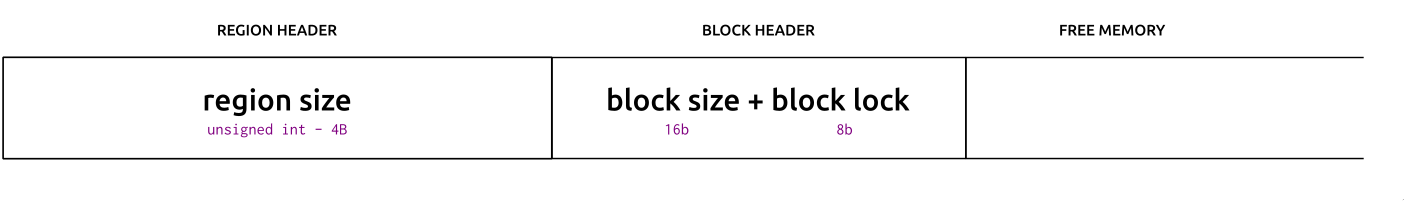
\includegraphics[width=\linewidth]{memory_init.png}
\end{figure}

\textbf{Region header} obsahuje informáciu o veľkosti celého regiónu, s ktorým budeme pracovať, a teda hneď aj obsadí 4B, a použiteľná pamäť sa zmenší.

\textbf{Block header} obsahuje obdobne informáciu o veľkosti bloku, a tzv. \textit{block lock}. Keďže zo zadania je jasné, že najväčši blok, ktorý sa budeme snažiť alokovať je 50000B, na uloženie veľkosti bloku stačí 16b, a teda ušetríme 2B oproti implementácii, ktorá by použila celý \textit{unsigned int}.

\newpage

Či je pamäť už obsadená si pamätáme v \textbf{block lock} - ak je zamknutá (block\_lock == 1), považujeme blok za alokovaný. Funkcia memory\_init teda nastaví block\_size na celkovú veľkosť - veľkosť hlavičky regiónu - veľkosť hlavičky bloku, teda celkovú veľkosť - 4 - 3, takže použiteľná pamäť je o 7B menšia (veľkosť slova je 1B)

Samotný región dostaneme od OS v podobe:
\begin{lstlisting}
	char* region = (char *) malloc(region_size);
\end{lstlisting}
a uložíme ho do globálnej premennej.

Nasledovne naň môžeme volať: 
\begin{lstlisting}
	memory_alloc();
	memory_free();
\end{lstlisting}

\textbf{memory\_alloc} dostane ako parameter veľkosť, ktorú cheme alokovať. Po zavolaní hľadá miesto pre blok takejto veľkosti metódou first fit. Ak je toto voľné miesto omnoho väčšie (a teda oplatí sa rozdeloť ho), rozdelíme ho na 2 menšie bloky, jeden presne veľkosti ktorú sme chceli alokovať + veľkosť hlavičky, druhé sa natiahne na celý zvyšok veľkosti. Ak je ale toto voľné miesto menšie než veľkosť na alokovanie + veľkosť hlavičky (samozrejme zároveň musí byť veľké minimálne veľkosť na alokovanie), pamäť nedelíme, miesto toho alokujeme trochu väčší blok. Nakoniec vrátime pointer na začiatok použiteľnej pamäte (pointer na hlavičku + veľkosť hlavičky).

\textbf{memory\_free} očakáva validný pointer ako vstup, a jednoducho prepíše v hlavičke block lock na 0. Keďže sa podľa zadania môžeme spoľahnúť, že vždy dostane validný pointer, nič viac tu riešiť netreba.

Na tomto mieste je aj vhodné spojiť prípadné za sebou idúce voľné bloky do jedného, takže aj prebehneme celý región, a ak sa takéto bloky nájdu, spojíme ich.

\newpage

\begin{lstlisting}
int memory_check (void *ptr)
{
	// calculate pointer to head
	char *head = (char *)(ptr - (HEADER_SIZE) );

	// is the pointer even in range?
	if ( !in_range(head) )
		return 0;

	// is the pointer allocated?
	char *tmp = region;
	while ( in_range(tmp) )
		if ( head == tmp && block_locked(tmp) )
			return 1;
		else
			tmp = next_block(tmp);

	return 1;
}
\end{lstlisting}

\textbf{memory\_check} slúži na zistenie, či daný pointer odkazuje na validný alokovaný blok pamäte. Zistíme to tak, že najprv vypočítame odkaz na hlavičku daného bloku, overíme či sa vypočítaný pointer vôbec nachádza v našom regióne, a ak áno, prebehneme región a skúšame nájsť daný poiner. Ak ho nájdeme, vrátime 1, inak vrátime 0.

\section*{Helpers}

Okrem zadaných funkcií sme si vytvorili aj pomocné funkcie, kvôli lepšej čitateľnosti kódu:
\begin{lstlisting}
while ( !can_alloc(ptr, size) ) // the block is locked or too small
{ ... 
\end{lstlisting}

a znovupoužiteľnosti:
\begin{lstlisting}
void gen_header (void *ptr, int size, int locked)
\end{lstlisting}

\section*{Testovanie a efektivita}

\textbf{memory\_alloc} má pri našom prístupe lineárnu časovú zložitosť - to znamená, že čím viac blokov máme alokovaných, tým dlhšie trvá alokovanie ďalšieho bloku. To očividne nie je najlepšie riešenie, a dalo by sa zefektívniť o čosi komplikovanejším prístupom. Ďalším problémom je taktiež fragmentácia - keďže používame first fit alokáciu, pri istých scénaroch nebude možné alokovať blok, na ktorý je dosť voľnej pamäte, len bude roztrúsená pomedzi alokované bloky.

\textbf{memory\_free} prebieha v konštantom čase - keďže stačí prísť na pointer na vstupe a odomknúť daný blok. Avšak po odomknutí prejdeme celú pamäť a hľadáme, či by sa nedali spojiť voľné bloky, čo prebieha v lineárnom čase.

\textbf{veľkosť hlavičky} je pomerne malá - len 3 slová, vďaka čomu dokážeme využiť zo 100B regiónu až 72B na dáta a 27B na hlavičky (pri blokoch veľkosti 8B).

\textbf{testovanie} sme previedli pre viacero scénarov. Najprv alokujeme malé slová rovnakej dĺžky do relatívne malých regiónov, kde nachádzame efektivitu okolo 70\%. Následne alokujeme malé slová rôznej dĺžky do malých regiónov. Ďalšie scénare zahŕňajú alokovanie veľkých slov nerovnakej dĺžky do veľkých blokov a alokovanie malých aj veľkých nerovnakých slov do regiónov veľkej dĺžky. Môžeme si všímnúť, že pri väčších slovách je efektivita vyššia, keďže stačí menej hlavičiek.

Dôkladne testovanie nám aj dokazuje, že alokované bloky nevychádzajú z rozsahu regiónu, neprekrývajú sa, a ani iným spôsobom si vzájomne neškodia.
\newpage


\end{document}
